\documentclass{beamer}

%\usepackage[utf8]{inputenc}
\usepackage{fontspec}
\usepackage{amsmath,amssymb,tikz-cd}
\usepackage{xcolor, xspace}

%\usefonttheme[onlymath]{serif}
%\usetheme{Warsaw}

\definecolor{darkblue}{HTML}{12335F}
\definecolor{myblue}{HTML}{00A2FF}

%--------------------------------------------------------------------------------
% Custom Template
%--------------------------------------------------------------------------------
\usecolortheme[named=myblue]{structure}

\setbeamertemplate{frametitle}{\vspace{5mm}\bfseries\insertframetitle}
\setbeamercolor{frametitle}{fg=darkblue}

\setbeamerfont{section in toc}{series=\bfseries}
\setbeamercolor{section in toc}{fg=darkblue}

\AtBeginEnvironment{theorem}{%
	\setbeamercolor{block title}{fg=white, bg=darkblue}
	\setbeamercolor{block body}{fg=black,bg=myblue!20}
}

%--------------------------------------------------------------------------------
% Custom Commands
%--------------------------------------------------------------------------------
\newcommand{\ER}{Erd\H{o}s R\'enyi\xspace}

%--------------------------------------------------------------------------------
% Fonts
%--------------------------------------------------------------------------------
\setsansfont{Helvetica Neue}

\begin{document}

%--------------------------------------------------------------------------------
% Title Page
%--------------------------------------------------------------------------------
{
\setbeamercolor{background canvas}{bg=darkblue}
\begin{frame}
	\bfseries
	{\color{white}
		\huge Percolation Phase Transitions on Dynamically Grown Graphs
	}
	\vspace{5mm}

	{\color{myblue}
		\large Braden Hoagland

		Advised by Rick Durrett
	}

	\vspace*{\fill}
	{\color{white}
		\small September 17, 2021
	}
\end{frame}
}

%--------------------------------------------------------------------------------
% Background
%--------------------------------------------------------------------------------
\section{Background}

{
\setbeamercolor{background canvas}{bg=darkblue}
\begin{frame}
        \bfseries
        {\color{white}
                \huge Background
        }
        \vspace{5mm}

	{\color{myblue}
		Dynamically grown graphs and percolation
	}
\end{frame}
}

\begin{frame}{Dynamically Grown Graphs}
	\begin{figure}[H]
		\centering
		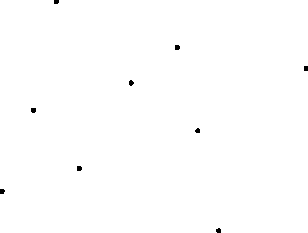
\includegraphics[scale=1]{fig/graph-1.pdf}
		%\caption{}
	\end{figure}
\end{frame}
\begin{frame}{Dynamically Grown Graphs}
        \begin{figure}[H]
                \centering
                \includegraphics[scale=1]{fig/graph-2.pdf}
                %\caption{}
        \end{figure}
\end{frame}
\begin{frame}{Dynamically Grown Graphs}
        \begin{figure}[H]
                \centering
                \includegraphics[scale=1]{fig/graph-3.pdf}
                %\caption{}
        \end{figure}
\end{frame}
\begin{frame}{Dynamically Grown Graphs}
        \begin{figure}[H]
                \centering
                \includegraphics[scale=1]{fig/graph-4.pdf}
                %\caption{}
        \end{figure}
\end{frame}
\begin{frame}{Dynamically Grown Graphs}
        \begin{figure}[H]
                \centering
                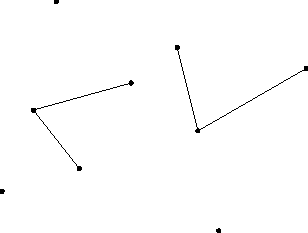
\includegraphics[scale=1]{fig/graph-5.pdf}
                %\caption{}
        \end{figure}
\end{frame}

\begin{frame}{Dynamically Grown Graphs}
	Every $t=1/n$ units of time, sample $m$ vertices.
	\vspace{5mm}

	Can only add edges between these $m$ vertices.
	\vspace{5mm}

	\pause
	Let $n\to \infty$.
\end{frame}

%-------------------
% Percolation
%-------------------
\subsection{Percolation}

\begin{frame}{Percolation}
	A \textit{giant component}: finite fraction of graph.
	\vspace{5mm}

	Percolation is the emergence of a giant component.
	\vspace{5mm}

	Lots of different behaviors.
\end{frame}

\begin{frame}
	\frametitle{Explosive Percolation}

	Simple rules: linear.
	\vspace{5mm}

	Prioritize merging smaller clusters: \textit{explosive percolation}.
\end{frame}

%--------------------------------------------------------------------------------
% Basic Results
%--------------------------------------------------------------------------------
\section{Basic Results}

{
\setbeamercolor{background canvas}{bg=darkblue}
\begin{frame}
        \bfseries
        {\color{white}
                \huge Basic Results
        }
        \vspace{5mm}

        {\color{myblue}
                Continuity of the phase transition and scaling behavior
        }
\end{frame}
}

%-------------------
% Continuity of the Phase Transition
%-------------------
\subsection{Continuity of the Phase Transition}

\begin{frame}
	\frametitle{Continuity of the Phase Transition}

	\textit{$\ell$-vertex rule}: choose $\ell$ vertices i.i.d., and you're only required to add an edge if all $\ell$ of them are in distinct clusters.
	\vspace{5mm}

	Riordan, R., and Warnke, L. (2012): continuous phase transition.
	\vspace{5mm}

	\pause
	Proof by contradiction...
\end{frame}

%-------------------
% Scaling Behavior
%-------------------
\subsection{Scaling Behavior}

\begin{frame}
	\frametitle{Scaling Behavior}

	For rules with continuous phase transitions, we see \textit{scaling behavior}.
	\vspace{5mm}

	Let $\delta = t-t_c$ and let $P(s, t)$ be the probability that a randomly chosen vertex has cluster size $s$ at time $t$. Then near $t_c$, there are constants $\tau$ and $\sigma$ such that
	\[
		P(s) = s^{1-\tau}f(s \delta^{1/\sigma}).
	\]
	\vspace{5mm}

	\pause
	{\color{myblue}\bfseries From now on, we assume scaling behavior.}
\end{frame}

\begin{frame}{Scaling Behavior}
	Let $S$ be the relative size of the giant component, and let
	\[
		\chi_k(t) = \sum_s s^{k} P(s, t).
	\] Then
	\[
		S \approx \delta^{\beta}, \quad\quad
		\chi_1(t) \approx \delta^{-\gamma}, \quad\quad
		\frac{\chi_k(t)}{\chi_{k-1}(t)}  \approx \delta^{-\Delta}
	\]
	These unknowns are called \textit{critical exponents}.
\end{frame}

\begin{frame}
	\frametitle{Scaling Relations}

	Goal: determine all critical exponents in terms of one unknown.
	\vspace{5mm}

	Why is this useful?
	\vspace{5mm}

	\pause
	What kinds of rules can we do this for?
\end{frame}

%--------------------------------------------------------------------------------
% 2-Choice Rules
%--------------------------------------------------------------------------------
\section{2-Choice Rules}

{
\setbeamercolor{background canvas}{bg=darkblue}
\begin{frame}
        \bfseries
        {\color{white}
                \huge 2-Choice Rules
        }
        \vspace{5mm}

        {\color{myblue}
		Generalizing rules with useful properties
        }
\end{frame}
}

\begin{frame}{2-Choice Rules}
	\begin{figure}[H]
		\centering
		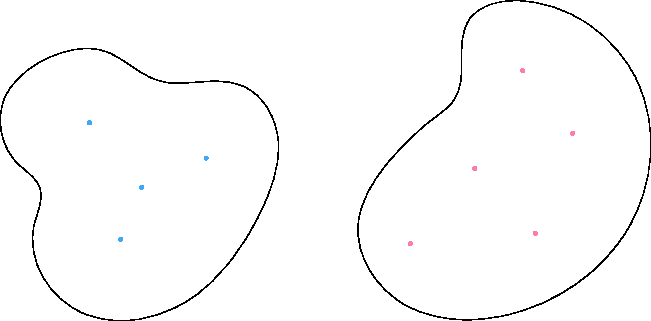
\includegraphics[scale=0.8]{fig/2choice-1.pdf}
		%\caption{}
	\end{figure}
\end{frame}
\begin{frame}{2-Choice Rules}
	\begin{figure}[H]
		\centering
		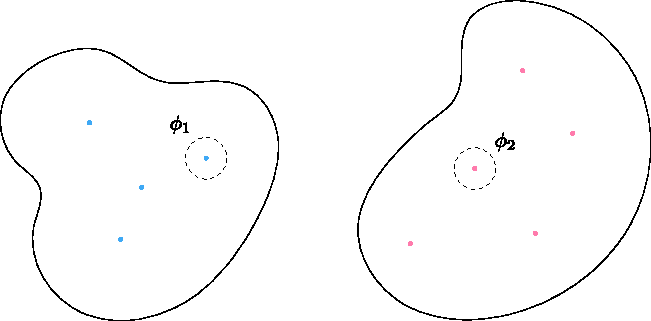
\includegraphics[scale=0.8]{fig/2choice-2.pdf}
		%\caption{}
	\end{figure}
\end{frame}
\begin{frame}{2-Choice Rules}
        \begin{figure}[H]
                \centering
                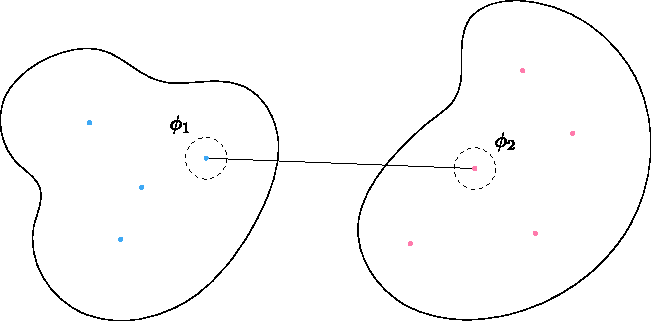
\includegraphics[scale=0.8]{fig/2choice-3.pdf}
                %\caption{}
        \end{figure}
\end{frame}

\begin{frame}{\ER}
	Pick two random vertices and add an edge between them.
	\vspace{5mm}

	\pause
	Percolation occurs after $t_c=1/2$.
	\vspace{5mm}

	$\beta=1$, so $S$ grows linearly near $t_c$.
\end{frame}

\begin{frame}{Minimizing Rules}
	\begin{figure}[H]
		\centering
		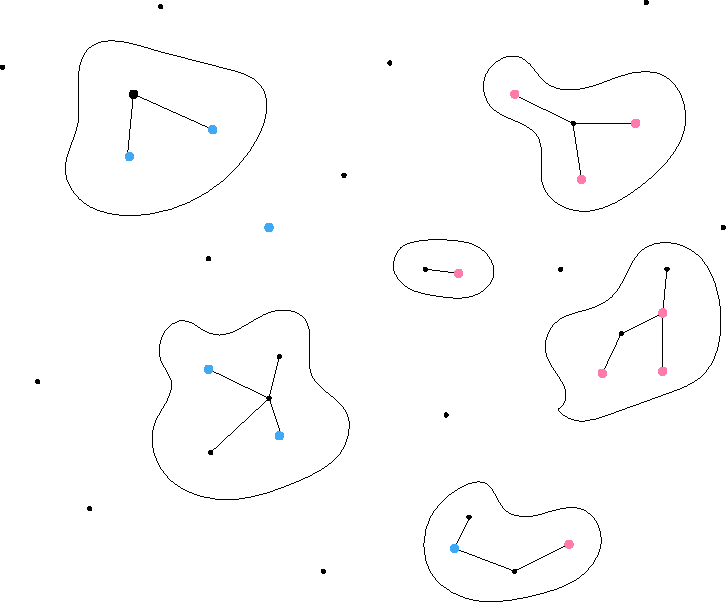
\includegraphics[scale=0.7]{fig/minimizing-1.pdf}
		%\caption{}
	\end{figure}
\end{frame}

\begin{frame}{Minimizing Rules}
	\begin{figure}[H]
		\centering
		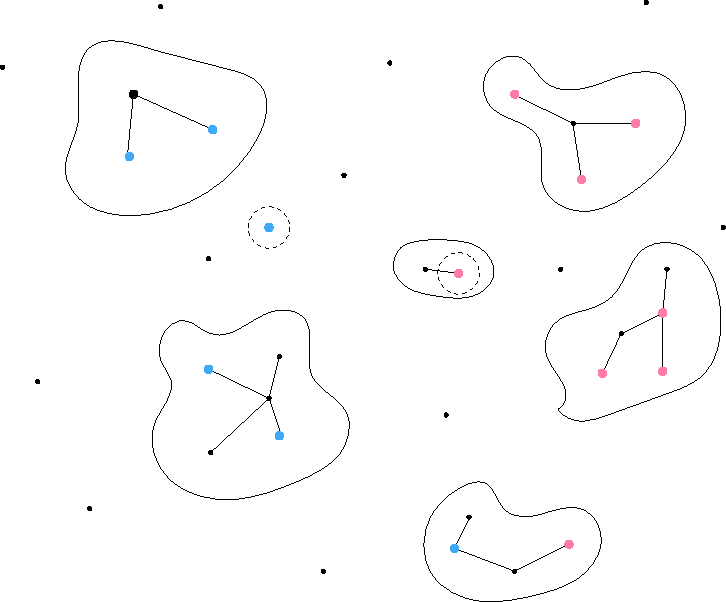
\includegraphics[scale=0.7]{fig/minimizing-2.pdf}
		%\caption{}
	\end{figure}
\end{frame}

\begin{frame}{Minimizing Rules}
        \begin{figure}[H]
                \centering
                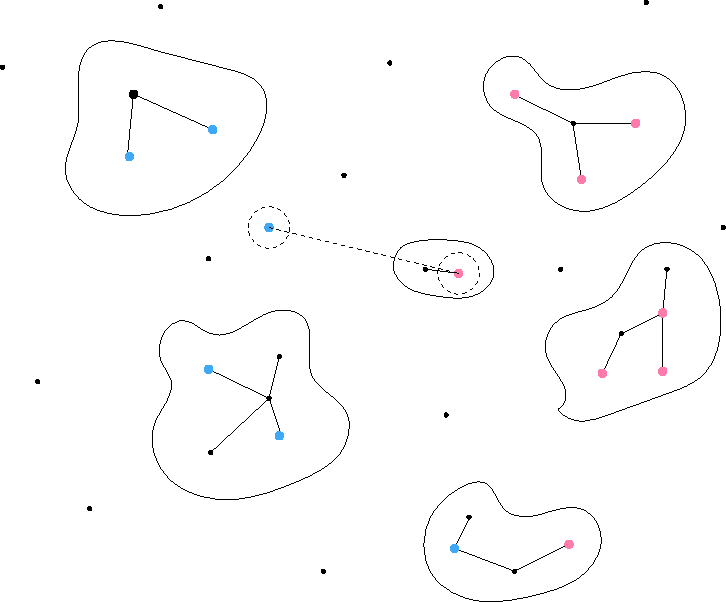
\includegraphics[scale=0.7]{fig/minimizing-3.pdf}
                %\caption{}
        \end{figure}
\end{frame}

\begin{frame}{da Costa}
	Minimizing rule with equal size groups.
	\vspace{5mm}

	Originally introduced to disprove Achlioptas' discontinuity conjecture.
	\vspace{5mm}

	Same as \ER when $m=1$. As $m\to \infty$,
	\[
	\beta\to 0, \quad\quad t_c \to 1.
	\]
\end{frame}

%-------------------
% Uniform Scaling
%-------------------
\subsection{Preliminary Results}

\begin{frame}{Finding the Critical Exponents}
	For any 2-choice rule, the quantity $\partial_{t}{S} $ has a simple form that can be explicitly calculated.
	\vspace{5mm}

	Near $t_c$, it will look like
	\[
	\delta^{a}+\delta^{b}+\delta^{c}+\cdots
	\] 
\end{frame}

\begin{frame}{Finding the Critical Exponents}
	\begin{theorem}
		For any 2-choice rule, there will be two dominating terms of $\partial_t S$ with the same order.
	\end{theorem}

	\pause
	\vspace{5mm}
	For all 2-choice rules, we can solve for all critical exponents in terms of $\beta$.
	
	\vspace{5mm}
	We also get the growth rate of the average cluster size.
\end{frame}

\begin{frame}{Minimizing Rules}
	\begin{align*}
		\gamma_a &= 1+(b-1)\beta, \\
		\gamma_b &= 1+(a-1)\beta, \\
		\gamma_{P} &= 1+(a+b-2)\beta, \\
		\frac{1}{\sigma} &= 1+(a+b-1)\beta, \\
		\tau &= \frac{\beta}{1+(a+b-1)\beta} +2.
	\end{align*}
\end{frame}

\begin{frame}{Asymptotics for Minimizing Rules}
	$\beta\to 0$ as $a,b \to \infty$.

	\vspace{5mm}
	\begin{theorem}
		$a \beta, b\beta\to 0$ as $a,b \to \infty$.
	\end{theorem}

	\pause
	\begin{align*}
		\gamma_{a}=\gamma_{b}=\gamma_{P}=\frac{1}{\sigma} &= 1, \\
		\tau &= 2.
	\end{align*}

	\vspace{5mm}
	\pause
	$\text{Var}(s) \to \delta^{-2}$.
\end{frame}

%--------------------------------------------------------------------------------
% Future Directions
%--------------------------------------------------------------------------------
\section{Future Directions}

{
\setbeamercolor{background canvas}{bg=darkblue}
\begin{frame}
        \bfseries
        {\color{white}
                \huge Future Directions
        }
\end{frame}
}

\begin{frame}{Future Directions}
	\begin{itemize}
		\item \ER is nice. Can we relate other rules to it?
			\begin{itemize}
				\item bounded size rules
				\item Universality classes
			\end{itemize}
		\item When is $t_c$?
			\begin{itemize}
				\item Bohman-Frieze variant
			\end{itemize}
		\item How fast is convergence to the asymptotic case?
		\item When does scaling behavior actually occur?
	\end{itemize}
\end{frame}


\end{document}
